\documentclass[a4paper,12pt]{article}
\usepackage[utf8]{inputenc}
\usepackage{amsmath}
\usepackage{amsfonts}
\usepackage{amssymb}
\usepackage{graphicx}

\numberwithin{equation}{section}
\renewcommand\thesubsection{\alph{subsection}}

%opening
\title{Quantum I HW5}
\author{Vince Baker}

\begin{document}

\maketitle

\section{Problem 1: Zeeman and Stark effects}
\subsection{}
The valence electron in a sodium atom will have nondegenerate N=3 states due to the screening effects of the lower-shell electrons.
With the 3P and 3D state energies lifted by 2 and 3 with respect to the 3S state, the $H_0$ matrix is: 
\begin{equation}
H_0=
\begin{bmatrix}
 0 & 0 & 0 & 0 & 0 & 0 & 0 & 0 & 0 \\
 0 & 2 & 0 & 0 & 0 & 0 & 0 & 0 & 0 \\
 0 & 0 & 2 & 0 & 0 & 0 & 0 & 0 & 0 \\
 0 & 0 & 0 & 2 & 0 & 0 & 0 & 0 & 0 \\
 0 & 0 & 0 & 0 & 3 & 0 & 0 & 0 & 0 \\
 0 & 0 & 0 & 0 & 0 & 3 & 0 & 0 & 0 \\
 0 & 0 & 0 & 0 & 0 & 0 & 3 & 0 & 0 \\
 0 & 0 & 0 & 0 & 0 & 0 & 0 & 3 & 0 \\
 0 & 0 & 0 & 0 & 0 & 0 & 0 & 0 & 3 \\
\end{bmatrix}
\end{equation}
\\
\subsection{}
With an external magnetic field applied along the z axis we look for the $L_z$ and $L_x$ operator elements.
Schwinger's isomorphism between the operators for two uncoupled harmonic oscillators and angular momentum operators gives us:
\begin{gather}
L_z(\ell^{'}=\ell, m^{'}=m)=m\\
L_z=
\begin{bmatrix}
 0 & 0 & 0 & 0 & 0 & 0 & 0 & 0 & 0 \\
 0 & 1 & 0 & 0 & 0 & 0 & 0 & 0 & 0 \\
 0 & 0 & 0 & 0 & 0 & 0 & 0 & 0 & 0 \\
 0 & 0 & 0 & -1 & 0 & 0 & 0 & 0 & 0 \\
 0 & 0 & 0 & 0 & 2 & 0 & 0 & 0 & 0 \\
 0 & 0 & 0 & 0 & 0 & 1 & 0 & 0 & 0 \\
 0 & 0 & 0 & 0 & 0 & 0 & 0 & 0 & 0 \\
 0 & 0 & 0 & 0 & 0 & 0 & 0 & -1 & 0 \\
 0 & 0 & 0 & 0 & 0 & 0 & 0 & 0 & -2 \\
\end{bmatrix}
\end{gather}
\\
\subsection{}
The matrix elements of $L_x$ can be calculated from the raising and lower operators $L^{\pm}$ by:
\begin{gather}
 L_+=L_x+iL_y\\
 L_-=L_x-iL_y\\
 L_x=\frac{1}{2}(L_++L_-)
\end{gather}
Again using Schwinger's harmonic oscillator isomorphism, we find:

\begin{gather}
L_+(\ell^{'}=\ell, m^{'}=m \pm 1)=\sqrt{(\ell-m)(\ell+m+1)}\\
L_-(\ell^{'}=\ell, m^{'}=m \pm 1)=\sqrt{(\ell-m)(\ell-m+1)}\\
L_x=\frac{1}{2}
\begin{bmatrix}
 0 & 0 & 0 & 0 & 0 & 0 & 0 & 0 & 0 \\
 0 & 0 & \sqrt{2} & 0 & 0 & 0 & 0 & 0 & 0 \\
 0 & \sqrt{2} & 0 & \sqrt{2} & 0 & 0 & 0 & 0 & 0 \\
 0 & 0 & \sqrt{2} & 0 & 0 & 0 & 0 & 0 & 0 \\
 0 & 0 & 0 & 0 & 0 & \sqrt{4} & 0 & 0 & 0 \\
 0 & 0 & 0 & 0 & \sqrt{4} & 0 & \sqrt{6} & 0 & 0 \\
 0 & 0 & 0 & 0 & 0 & \sqrt{6} & 0 & \sqrt{6} & 0 \\
 0 & 0 & 0 & 0 & 0 & 0 & \sqrt{6} & 0 & \sqrt{4} \\
 0 & 0 & 0 & 0 & 0 & 0 & 0 & \sqrt{4} & 0 \\
\end{bmatrix}
\end{gather}
The energy spectrum of $L_z$ and $L_x$ are identical and are shown below:\\
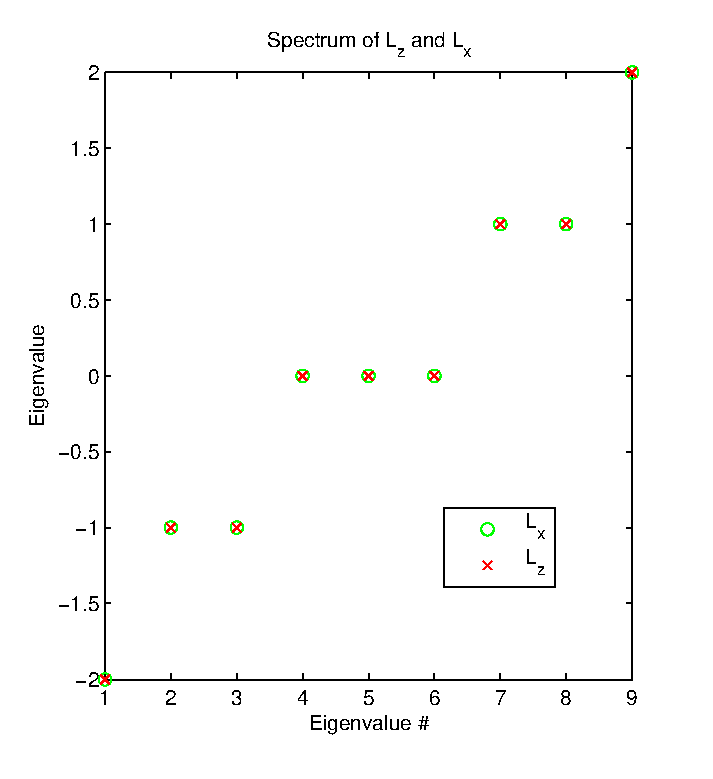
\includegraphics{Lx_Lz}
\\
\subsection{}
A uniform electric field is applied parallel to the z axis.
With $z=r\cos\theta$ we use the properties of the spherical harmonics as a complete orthonormal basis.
We find the radial contribution is $\frac{-3}{2}n\sqrt{n^2-\ell^2}$. 
Since $\cos\theta=Y_0^1$, we can look up the spherical harmonic integrals.
We find the angular contribution is $\sqrt{\frac{(\ell+m)(\ell-m)}{(2\ell+1)(2\ell-1)}}$.
The Hamiltonian is:
\begin{equation}
-e|E|z=
\begin{bmatrix}
 0 & 0 & 1.633 & 0 & 0 & 0 & 0 & 0 & 0 \\
 0 & 0 & 0 & 0 & 0 & 1 & 0 & 0 & 0 \\
 1.633 & 0 & 0 & 0 & 0 & 0 & 1.1547 & 0 & 0 \\
 0 & 0 & 0 & 0 & 0 & 0 & 0 & 1 & 0 \\
 0 & 0 & 0 & 0 & 0 & 0 & 0 & 0 & 0 \\
 0 & 1 & 0 & 0 & 0 & 0 & 0 & 0 & 0 \\
 0 & 0 & 1.1547 & 0 & 0 & 0 & 0 & 0 & 0 \\
 0 & 0 & 0 & 1 & 0 & 0 & 0 & 0 & 0 \\
 0 & 0 & 0 & 0 & 0 & 0 & 0 & 0 & 0 \\
\end{bmatrix}
\end{equation}

\subsection{}
The energy spectrum of the sodium atom in electric and magnetic fields as a function of magnetic field angle $\theta$ is shown below:\\
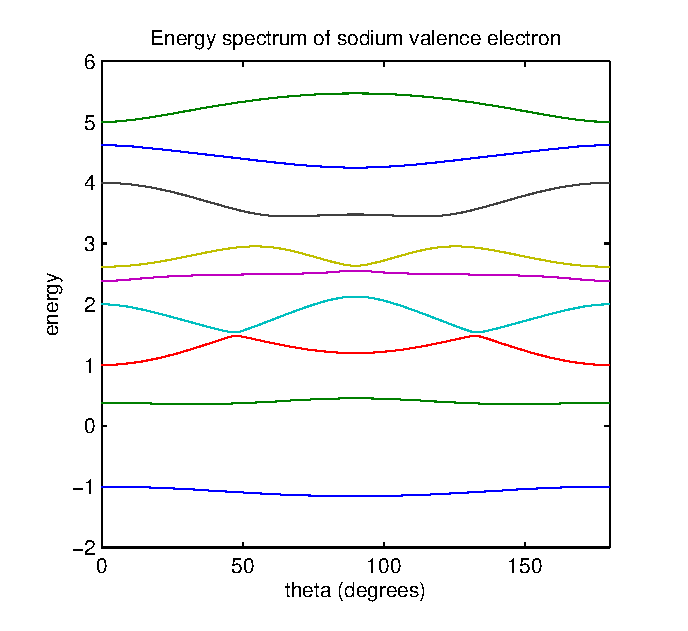
\includegraphics{Na_spectrum}
\\
\subsection{}
We explore the shape of the 2nd and 3rd excited states as the magnetic field direction is rotated with respect to the electric field.
The electron angular momentum will tend to align with the magnetic field, while the electron-proton dipole moment will tend to align with the electric field.
Inspecting the eigenvectors of the total Hamiltonian when $\theta=0$ we see that the 2nd excited state is correlated entirely with the 5th mode ($\ell=2,\ m=2$).
$Y_2^2(\theta, \phi)\sim \sin^2 \theta\ e^{i2\phi}$, so it has 4 lobes sticking into the x/y plane with a $\sin^2$ shape. 
The energy levels of the 2nd and 3rd excited states become almost degenerate at the kink points (approximately 45 degrees) where the electric and magnetic field effects cancel each other.


\end{document}
